%% Status: 2015-12-30 Some parts collected from wiki.
%% TODO: Describe StellariumScope plugin
\chapter{Stellarium at the Telescope}
\label{ch:atTheTelescope}

Stellarium is great for indoor use on the desktop, but it is also very
useful outdoors under the real sky, and several plugins enhance its
usability particularly for observers.

Two plugins are bundled with Stellarium which are designed to be used
at the telescope: Oculars (section~\ref{sec:plugins:Oculars}), which
provides field of view hints for telescopes, oculars and sensors, and
TelescopeControl (section~\ref{sec:plugins:TelescopeControl}), which
allows you to send GOTO commands to many motorized telescopes. Other
goto telescopes are supported by an external plugin which you must
install separately: StellariumScope
(section~\ref{sec:plugins:StellariumScope}).

In addition, the Observability plugin (section~\ref{sec:plugins:Observability})
can be used for planning the best times to observe your favourite
objects.

\section{Oculars Plugin}
\label{sec:plugins:Oculars}

This places a window on the screen that corresponds to the view
through a telescope or on a camera. It reads from an editable data
base.

When this plug in is active a circular view will appear around the
selected object depicting what would be seen by the viewing object. On
the top right hand side of the screen a menu will appear that can be
used to select the viewing device, e.g., Camera, Eyepiece, Barlow type
lenses, etc. This menu is filled with items from the \file{ocular.ini}
file in the \file{modules/oculars} folder. This file can be edited
from the Plugin's menu screen or with a text editor.

%TODO: Details?

\newpage
\section{TelescopeControl Plugin}
\label{sec:plugins:TelescopeControl}

This plugin provides a simple control mechanism for motorised
telescope mounts. The user selects an object (i.e.\ by clicking on
something -- a planet, a star etc.) and presses the telescope go-to
key, and the telescope will be guided to the object.

Multiple telescopes may be controlled simultaneously. 

% %TODO Details?
% 
% The control interface uses the Meade or the Celestron protocol and
% most telescopes use either one or the other so many different brands
% of telescopes can be controlled. There is a third party Telescope
% control system going under the name of ASCOM. They provide an
% interface to stellarium and then translate the control into many other
% forms (see section~\ref{sec:plugins:StellariumScope}).
% 
%% GZ Taken from the plugins help page, only slightly reformatted.

\paragraph{WARNING}\emph{Stellarium cannot prevent your
telescope from being pointed at the Sun. It is up to you to ensure
proper filtering and safety measures are applied!}

Never point your telescope at the Sun without a proper solar filter
installed. The powerful light amplified by the telescope WILL cause
\emph{irreversible damage} to your eyes and/or your equipment.

Even if you don't do it deliberately, a slew during daylight hours may
cause your telescope to point at the sun on its way to the given
destination, so it is strongly recommended to avoid using the
telescope control feature before sunset without appropriate
protection.



\subsection{Abilities and limitations}
\label{sec:sec:plugins:TelescopeControl:Linitaitons}

This plug-in allows Stellarium to send only 'slew' ('go to') commands
to the device and to receive its current position. It cannot issue any
other commands, so users should be aware of the possibility for mount
collisions and similar situations. (To abort a slew, you can start
another one to a safe position.)

Currently this plug-in does not allow satellite tracking, and is not
very suitable for lunar or planetary observations.

\subsection{Using this plug-in}
\label{sec:plugins:TelescopeControl:using}

Here are two general ways to control a device with this plug-in, depending on the situation:
\begin{description}
\item[DIRECT CONNECTION] A device supported by the plug-in is
  connected with a cable to the computer running Stellarium

\item[INDIRECT CONNECTION]\mbox{\ } % \\
  \begin{description}
  \item[local] A device is connected to the same computer but it is
    driven by a stand-alone telescope server program or a third-party
    application that can 'talk' to Stellarium;

  \item[remote] A device is connected to a remote computer and the
    software that drives it can 'talk' to Stellarium over the network;
    this software can be either one of Stellarium's stand-alone
    telescope servers, or a third party application.
  \end{description}
\end{description}
Most older telescopes use cables that connect to a serial port
(RS-232), the newer ones use USB (Universal Serial Bus). On Linux and
Max OS X, both cases are handled identically by the plug-in. On
Windows, a USB connection may require a 'virtual serial port'
software, if it is not supplied with the cable or the telescope. Such
a software creates a virtual ('fake') COM port that corresponds to the
real USB port so it can be used by the plug-in. On all three
platforms, if the computer has no 'classic' serial ports and the
telescope can connect only to a serial port, a serial-to-USB
(RS-232-to-USB) adapter may be necessary.

Telescope set-up (setting geographical coordinates, performing
alignment, etc.) should be done before connecting the telescope to
Stellarium.

\subsection{Main window ('Telescopes')}

The plug-in's main window can be opened:
\begin{itemize}
\item By pressing the \button{configure} button for the plug-in in the
  \menu{Plugins} tab of Stellarium's Configuration window (opened by
  pressing \keys{F2} or the \guibutton[0.35]{2}{btd_config} button in the left toolbar).
\item By pressing the \button{Configure telescopes...} button in the \menu{Slew to}
  window (opened by pressing \keys{\ctrl+0} or the respective button on the
  bottom toolbar).
\end{itemize}

\noindent The \menu{Telescopes} tab displays a list of the telescope connections that have been set up:

\begin{itemize}
\item The \emph{number (\#)} column shows the number used to control this
  telescope. For example, for telescope \#2, the shortcut is
  \keys{\ctrl+2}.
\item The \emph{Status} column indicates if this connection is
  currently active or not. Unfortunately, there are some cases in
  which 'Connected' is displayed when no working connection exists.
\item The \emph{Type} field indicates what kind of connection is this:
  \begin{description}
  \item[virtual] means a virtual telescope
  \item[local, Stellarium] means a
    DIRECT connection to the telescope (see above)
  \item[local, external] means an INDIRECT connection to a program
    running on the same computer
  \item[remote, unknown] means an INDIRECT connection over a network
    to a remote machine.
  \end{description}
\end{itemize}

\noindent To set up a new telescope connection, press the \button{Add} button. To modify
the configuration of an existing connection, select it in the list and
press the \button{Configure} button. In both cases, a telescope connection
configuration window will open.



\subsection{Telescope configuration window}

\paragraph{Connection type}
The topmost field represents the choice between the types of connections (see section~\ref{sec:plugins:TelescopeControl:using}):
Telescope controlled by:
\begin{description}
\item[Stellarium, directly through a serial port] is the DIRECT case
\item[External software or a remote computer] is the INDIRECT case
\item[Nothing, just simulate one (a moving reticle)] is a \emph{virtual telescope} (no connection)
\end{description}

\paragraph{Telescope properties}

\begin{description}
\item[Name] is the label that will be displayed on the screen next to
  the telescope reticle.
\item[Connection delay] If the movement of the telescope reticle on
  the screen is uneven, you can try increasing or decreasing this
  value.
\item[Coordinate system] Some Celestron telescopes have had their
  firmware updated and now interpret the coordinates they receive as
  coordinates that use the equinox of the date (EOD, also known as
  JNow), making necessary this setting.
\item[Start/connect at startup] Check this option if you want
  Stellarium to attempt to connect to the telescope immediately after
  it starts. Otherwise, to start the telescope, you need to open the
  main window, select that telescope and press the \button{Start/Connect}
  button.
\end{description}

\paragraph{Device settings}
This section is active only for DIRECT connections (see above).

\begin{description}
\item[Serial port] sets the serial port used by the telescope.  There
  is a pop-up box that suggests some default values:
  \begin{itemize}
  \item On Windows, serial ports \texttt{COM1} to \texttt{COM10}
  \item On Linux, serial ports \texttt{/dev/ttyS0} to
    \texttt{/dev/ttyS3} and USB ports \texttt{/dev/ttyUSB0} to
    \texttt{/dev/ttyUSB3}
  \item On Mac OS X, the list is empty as it names its ports in a
    peculiar way.
  If you are using an USB cable, the default serial port of your
  telescope most probably is not in the list of suggestions.  To list
  all valid serial port names in Mac OS X, open a terminal and type:

\begin{commands}
  ls /dev/*
\end{commands}
%
This will list all devices, the full name of your serial port should
be somewhere in the list (for example,
\texttt{/dev/cu.usbserial-FTDFZVMK}).
\end{itemize}

\item[Device model]: see~\ref{sec:plugins:TelescopeControl:supported} Supported devices.
\end{description}

\paragraph{Connection settings}
Both fields here refer to INDIRECT connections, which implies communication over a network (TCP/IP). 
\begin{description}
\item[Host] can be either a host name or an IPv4 address such as
  '127.0.0.1'.  The default value of 'localhost' means 'this
  computer'. 

  Modifying the default host name value makes sense only if you are
  attempting a remote connection over a network. In this case, it
  should be the name or IP address of the computer that runs a program
  that runs the telescope.
\item[Port] refers to the TCP port used for communication. The default
  value depends on the telescope number and ranges between 10001 and
  10009.
\end{description}
%
Both values are ignored for DIRECT connections.

\paragraph{User Interface Settings: Field of view indicators}

A series of circles representing different fields of view can be added
around the telescope marker. This is a relic from the times before the
Oculars plug-in (see~\ref{sec:plugins:Oculars}) existed.

Activate the 'Use field of view indicators' option, then enter
a list of values separated with commas in the field below. The values
are interpreted as degrees of arc.

These marks can be used in combination with a virtual telescope to
display a moving reticle with the Telrad circles.


\subsubsection{'Slew telescope to' window}

The \menu{Slew telescope to} window can be opened by pressing \keys{\ctrl+0} or the respective button in the bottom toolbar.

It contains two fields for entering celestial coordinates, selectors
for the preferred format (Hours-Minutes-Seconds,
Degrees-Minutes-Seconds, or Decimal degrees), a drop-down list and two
buttons.

The drop-down list contains the names of the currently connected
devices. If no devices are connected, it will remain empty, and the
\button{Slew} button will be disabled.

Pressing the \button{Slew} button slews the selected device to the selected set
of coordinates. See the section about keyboard commands below for
other ways of controlling the device.

Pressing the \button{Configure telescopes\ldots} button opens the main window of
the plug-in.

TIP: Inside the 'Slew' window, underlined letters indicate that
pressing \keys{\Alt + underlined letter} can be used instead of
clicking. For example, pressing \keys{\Alt+S} is equivalent to
clicking the \button{Slew} button, pressing \keys{\Alt+E} switches to
decimal degree format, etc.


\subsubsection{Sending commands}

Once a telescope is successfully started/connected, Stellarium
displays a telescope reticle labelled with the telescope's name on its
current position in the sky. The reticle is an object like every other
in Stellarium - it can be selected with the mouse, it can be tracked
and it appears as an object in the 'Search' window.

To point a device to an object: Select an object (e.g. a star) and
press the number of the device while holding down the \keys{\ctrl} key. (For
example, \keys{\ctrl+1} for telescope \#1.) This will move the telescope to the
selected object.

To point a device to the center of the view: Press the number of the
device while holding down the Alt key. (For example, \keys{\Alt+1} for
telescope \#1.) This will slew the device to the point in the center of
the current view. (If you move the view after issuing the command, the
target won't change unless you issue another command.)

To point a device to a given set of coordinates: Use the \menu{Slew to} window (press \keys{\ctrl+0}).

\subsection{Supported devices}
\label{sec:plugins:TelescopeControl:supported}

All devices listed in the 'Device model' list are convenience
definitions using one of the two built-in interfaces: the Meade LX200
(the Meade Autostar controller) interface and the Celestron NexStar
interface.

The device list contains the following:
\begin{description}
\item[Celestron NexStar (compatible)] Any device using the NexStar
  interface.
\item[Losmandy G-11] A computerized telescope mount made by Losmandy
  (Meade LX-200/Autostar interface).
\item[Meade Autostar compatible] Any device using the LX-200/Autostar
  interface.
\item[Meade ETX-70 (\#494 Autostar, \#506 CCS)] The Meade ETX-70
  telescope with the \#494 Autostar controller and the \#506 Connector
  Cable Set. According to the tester, it is a bit slow, so its default
  setting of 'Connection delay' is 1.5 seconds instead of 0.5 seconds.
\item[Meade LX200 (compatible)] Any device using the LX-200/Autostar
  interface.
\item[Sky-Watcher SynScan AZ mount] The Sky-Watcher SynScan AZ GoTo
  mount is used in a number of telescopes.
\item[Sky-Watcher SynScan (version 3 or later)] SynScan is also the
  name of the hand controller used in other Sky-Watcher GoTo mounts,
  and it seems that any mount that uses a SynScan controller version
  3.0 or greater is supported by the plug-in, as it uses the NexStar
  protocol.
\item[Wildcard Innovations Argo Navis (Meade mode)] Argo Navis is a
  'Digital Telescope Computer' by Wildcard Innovations. It is an
  advanced digital setting circle that turns an ordinary telescope
  (for example, a dobsonian) into a 'Push To'' telescope (a telescope
  that uses a computer to find targets and human power to move the
  telescope itself). Just don't forget to set it to Meade
  compatibility mode and set the baud rate to 9600B1.
\end{description}


\subsubsection{Virtual telescope}
If you want to test this plug-in without an actual device connected to
the computer, choose ``Nothing, just simulate one (a moving reticle)'' in
the \menu{Telescope controlled by:} field. It will show a telescope reticle
that will react in the same way as the reticle of a real telescope
controlled by the plug-in.  See the section above about field of view
indicators for a possible practical application (emulating 'Telrad'
circles).  

%% We don't neeed this remark any longer after 5 years...
%This feature is equivalent to the 'Dummy' type of telescope
%supported by Stellarium's original telescope control feature.



\newpage
\section{StellariumScope plugin}
\label{sec:plugins:StellariumScope}
StellariumScope is a free add-on that enables you to control your telescope with Stellarium. 

\begin{figure}[htp]
\begin{center}
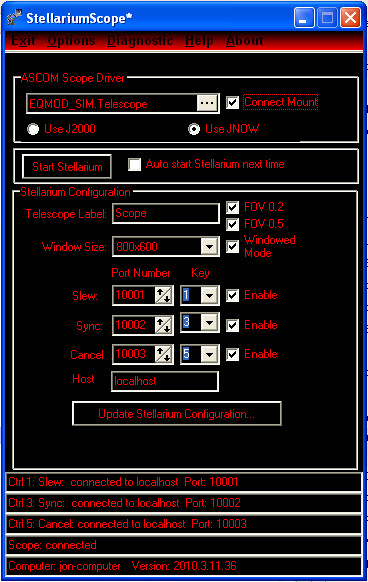
\includegraphics[width=0.85\linewidth]{StellariumScopeFullWindow.jpg}
\end{center}
\label{fig:StellariumScopeFullWindow}
\caption{StellariumScope interface}
\end{figure}


\paragraph{Features}
\begin{itemize}
\item Provides an interface between Stellarium and the ASCOM telescope drivers.
\item Provides the ability to both ``Sync'' and ``Slew'' the
  telescope. It's also possible to issue a stop/cancel command from
  Stellarium.
\item You can easily host Stellarium on one computer linked to another
  control computer that hosts the telescope driver.
\item The installation program will automatically install the
  documentation, but the link to the documentation is provided
  here\footnote{WHERE?} so you can read it before installation.
\item There are earlier releases still available on the downloads page on
  Welsh Dragon Computing site.
\end{itemize}

The original StellariumScope program was designed and implemented by
Scott of ByteArts and is still available for
download\footnote{\url{http://www.bytearts.com/stellarium/}}. If you
have difficulties with the releases available on the Welsh Dragon
Computing
site\footnote{\url{http://welshdragoncomputing.ca/x/index.php/home/stellariumscope/about-stellariumscope}},
you may want to consider using the original version.


Figure~\ref{fig:StellariumScopeFullWindow} shows the interface and
some of the options.  Use this application (like all software that
controls your mount) with supervision of your mount's movements.

\subsection{Configure StellariumScope}
\label{sec:plugins:StellariumScope:configure}
TODO...
\subsection{Download StellariumScope}
TODO...

\newpage
\section{Observability Plugin}
\label{sec:plugins:Observability}

This Plugin  analyzes the observability of the selected object (or the
screen center, if no object is selected). The plugin can show rise,
transit, and set times, as well as the best epoch of the year (i.e.,
largest angular separation from the Sun), the date range when the
source is above the horizon at dark night, and the dates of Acronychal
and Cosmical rise/set.  Ephemerides of the Solar-System objects and
parallax effects are taken into account.

\subsection*{Explanation of some parameters}

\begin{description}
\item[Sun altitude at twilight] Any celestial object will be
  considered visible when the Sun is below this altitude. The altitude
  at astronomical twilight ranges usually between -12 and -18
  degrees. This parameter is only used for the estimate of the range
  of observable epochs (see below).
\item[Horizon altitude] Minimum observable altitude (due to mountains,
  buildings, or just a limited telescope mount).
%% TODO: This should be replaced by the direct interaction with / evaluation of the landscape!!!
\item[Today ephemeris] Self-explanatory. The program will show the
  rise, set, and culmination (transit) times. The exact times for
  these ephemeris are given in two ways: as time spans (referred to
  the current time) and as clock hours (in local time).
\item[Acronychal/Cosmical/Heliacal rise/set] The days of Cosmical
  rise/set of an object are estimated as the days when the object
  rises (or sets) together with the rise/set of the Sun. The exact
  dates of these ephemeris depend on the Observer's location. On the
  contrary, the Acronycal rise (or set) happens when the star
  rises/sets with the setting/rising of the Sun (i.e., opposite to the
  Sun). On the one hand, it is obvious that the source is hardly
  observable (or not observable at all) in the dates between Cosmical
  set and Cosmical rise. On the other hand, the dates around the
  Acronychal set and rise are those when the altitude of the celestial
  object uses to be high when the Sun is well below the horizon (hence
  the object can be well observed). The date of Heliacal rise is the
  first day of the year when a star becomes visible. It happens when
  the star is close to the eastern horizon roughly before the end of
  the astronomical night (i.e., at the astronomical twilight). In the
  following nights, the star will be visibile during longer periods of
  time, until it reaches its Heliacal set (i.e., the last night of the
  year when the star is still visible). At the Heliacal set, the star
  sets roughly after the beginning of the astronomical night.
\item[Largest Sun separation] Happens when the angular separation
  between the Sun and the celestial object are maximum. In most cases,
  this is equivalent to say that the Equatorial longitudes of the Sun
  and the object differ by 180 degrees, so the Sun is in opposition to
  the object. When an object is at its maximum possible angular
  separation from the Sun (no matter if it is a planet or a star), it
  culminates roughly at midnight, and on the darkest possible area of
  the Sky at that declination. Hence, that is the 'best' night to
  observe a particular object.
\item[Nights with source above horizon] The program computes the range
  of dates when the celestial object is above the horizon at least
  during one moment of the night. By 'night', the program considers
  the time span when the Sun altitude is below that of the twilight
  (which can be set by the user; see above). When the objects are
  fixed on the sky (or are exterior planets), the range of observable
  epochs for the current year can have two possible forms: either a
  range from one date to another (e.g., 20 Jan to 15 Sep) or in two
  steps (from 1 Jan to a given date and from another date to 31
  Dec). In the first case, the first date (20 Jan in our example)
  shall be close to the so-called 'Heliacal rise of a star' and the
  second date (15 Sep in our example) shall be close to the 'Heliacal
  set'. In the second case (e.g., a range in the form 1 Jan to 20 May
  and 21 Sep to 31 Dec), the first date (20 May in our example) would
  be close to the Heliacal set and the second one (21 Sep in our
  example) to the Heliacal rise. More exact equations to estimate the
  Heliacal rise/set of stars and planets (which will not depend on the
  mere input of a twilight Sun elevation by the user) will be
  implemented in future versions of this plugin.
\item[Full Moon] When the Moon is selected, the program can compute
  the exact closest dates of the Moon's opposition to the Sun.
\end{description}

\subsection*{Author}
\label{sec:plugins:Observability:author}
This plugin has been contributed by Ivan Marti-Vidal (Onsala Space Observatory)\footnote{\url{mailto:i.martividal@gmail.com}} with some advice by Alexander Wolf and Georg Zotti.




%%% Local Variables: 
%%% mode: latex
%%% TeX-master: "guide"
%%% End: 

